\chapter{Implementazione}
\label{cha:implementazione}
In questo Capitolo viene descritta la fase di implementazione del sistema, che comprende lo sviluppo in accordo ai requisiti individuati, l'integrazione con il sistema implementato da Digicando ed il testing.

\section{Tecnologie utilizzate}
Per lo sviluppo del sistema sono state utilizzate le migliori tecnologie disponibili per lo sviluppo di smart contracts su blockchain Ethereum. Tutte le tecnologie utilizzate sono open-source, seguendo la filosofia della blockchain Ethereum, e sviluppate da una community di sviluppatori. Le principali sono:
\begin{itemize}
    \item \emph{Linguaggio di programmazione Solidity}: un linguaggio di programmazione ad alto livello orientato agli oggetti per lo sviluppo di smart contracts \cite{solidity-documentation}.
    \item \emph{Truffle}: un ambiente di sviluppo, un framework per il testing ed un insieme di risorse per la blockchain Ethereum \cite{trufflesuite}.
    \item \emph{Ganache}: uno strumento per creare blockchain Ethereum personali, utilizzabili per pubblicare contratti durante il loro sviluppo e condurre dei test \cite{trufflesuite}.
\end{itemize}

\section{I contratti}
\label{sec:contratti}
Il sistema di gestione dei ruoli è stato sviluppato nel linguaggio di programmazione ad alto livello per blockchain Ethereum \emph{Solidity}. Il sistema sviluppato è composto da due contratti:
\begin{itemize}
    \item \emph{ClaimsRegister}: memorizza i ruoli emessi.
    \item \emph{ClaimsManagement}: permette di gestire delle strutture organizzative dei ruoli gerarchiche e complesse.
\end{itemize}

\subsection{ClaimsRegister}
\label{claims-register}
Funge da registro per la memorizzazione di ruoli, chiamati \emph{claim}, con associato un valore da un emettitore ad un ricevitore. Si è scelto di utilizzare la parola \emph{claim} e non \emph{role} per mantenere una maggiore genericità e rendere il sistema più versatile. In pratica, una claim è una tupla formata da un emettitore, un ricevitore, la chiave della claim ed il relativo valore. Ogni indirizzo può emettere ruoli ad ogni indirizzo, infatti non è presente alcuna logica di controllo sui ruoli e la loro emissione ed il registro non conosce il significato dei ruoli. Spetterà alle applicazioni che utilizzeranno il registro implementare i meccanismi di controllo e dare un significato ai ruoli. Il contratto implementa due funzioni, per l'aggiunta e la rimozione dei ruoli.

Questo contratto, da solo, permette di gestire delle strutture organizzative dei ruoli ad un livello dove ogni utente ha gli stessi diritti degli altri e può rimuovere ed aggiungere utenti.

\paragraph{Registro di claim}
Il registro è un \texttt{mapping}, cioè una \emph{tabella hash} nel linguaggio Solidity, che memorizza un valore associato a tre chiavi.

\noindent
\begin{lstlisting}[language=Solidity]
    // emitter => receiver => claim => value
    mapping(address => mapping(address => mapping(bytes32 => bytes32))) public registry;
\end{lstlisting}

Le chiavi della tabella sono, in ordine:
\begin{itemize}
    \item \emph{Emitter}: è l'indirizzo Ethereum che emette il ruolo.
    \item \emph{Receiver}: è l'indirizzo Ethereum che riceve il ruolo.
    \item \emph{Claim}: è un array di 32 bytes che rappresenta la chiave di un ruolo. Un possibile metodo per l'identificazione di una chiave adeguata per un ruolo è calcolare l'hash di una stringa che descriva il ruolo.
\end{itemize}
Il valore \emph{value} associato alle tre chiavi è nuovamente un array di 32 bytes e rende il registro molto flessibile e versatile quando utilizzato da un'applicazione. Il valore, infatti, può essere utilizzato di base per memorizzare un valore booleano, ma un'applicazione può utilizzarlo per memorizzare informazioni con significati più ampi.

\paragraph{Metodi}
Il contratto implementa due metodi: uno per l'aggiunta e uno per la rimozione di claim.

\noindent
\begin{lstlisting}[language=Solidity]
    function setClaim(address receiver, bytes32 claim, bytes32 value)
        public
    {
        registry[msg.sender][receiver][claim] = value;
    }
\end{lstlisting}
Emette una claim dall'indirizzo che chiama la funzione ad un ricevitore specificato.

\noindent
\begin{lstlisting}[language=Solidity]
    function removeClaim(address receiver, bytes32 claim)
        public
    {
        delete(registry[msg.sender][receiver][claim]);
    }
\end{lstlisting}
Rimuove una claim precedentemente emessa dall'indirizzo che chiama la funzione ad un ricevitore specificato.

L'utilizzo di \texttt{msg.sender} nell'identificazione dell'emettitore nei due metodi assicura che solamente il possessore della chiave privata associata ad un indirizzo possa emettere e rimuovere claim con tale indirizzo.

\subsection{ClaimsManagement}
\label{claims-management}
Questo contratto implementa una funzione per il controllo della validità di catene di claim. Una catena di claim è valida solamente se ogni claim al suo interno esiste nel registro e se valgono le seguenti regole:
\begin{itemize}
    \item La prima claim è emessa da un indirizzo, chiamato \emph{root}, ad un ricevitore.
    \item Ogni claim successiva è emessa dal ricevitore della precedente.
\end{itemize}

Il contratto non memorizza le catene di claim, ma permette solamente il controllo della loro validità. Spetta alle applicazioni mantenere con delle strutture dati apposite. Il sistema permette la creazione ed il mantenimento di strutture organizzative gerarchiche complesse e ammette la presenza di più indirizzi \emph{radice} e la possibilità per un indirizzo di ricevere la stessa claim da più emettitori.

\begin{figure}[ht!]
    \centering
    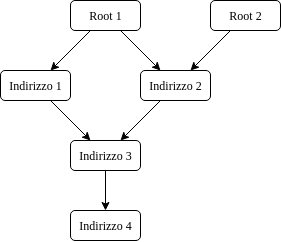
\includegraphics[scale=0.75]{img/gerarchia.png}
    \caption{Esempio di gerarchia complessa}
    \label{fig:gerarchia}
\end{figure}

\paragraph{Il metodo}
La funzione riceve in ingresso tre vettori:
\begin{itemize}
    \item \emph{chain}: la catena di utenti, ordinati dall'ultimo ricevitore alla root.
    \item \emph{claims}: la catena delle chiavi delle claim, dall'ultima alla prima.
    \item \emph{values}: la catena dei valori delle claim, dall'ultimo al primo.
\end{itemize}

La funzione effettua, per prima cosa, dei controlli sulle lunghezze dei vettori passati come parametri. Se i controlli vengono rispettati, la funzione procede a ciclare e verificare le claim della catena. Se una claim non risulta valida nel registro, la funzione ritorna \texttt{false}, se tutte le claim sono verificate ritorna \texttt{true}.

\noindent
\begin{lstlisting}[language=Solidity]
    function checkClaims(address[] memory chain, bytes32[] memory claims, bytes32[] memory values)
        public
        view
        returns (bool)
    {
        require(claims.length == chain.length - 1, "The length of the arrays is wrong");
        require(claims.length == values.length, "The length of the arrays is wrong");
    
        for(uint i = 0; i < chain.length - 1; i++){
            if(register.registry(chain[i + 1], chain[i], claims[i]) != values[i]) {
                return false;
            }
        }
    
        return true;
    }
\end{lstlisting}

\section{Integrazione}
Il processo di integrazione del nuovo sistema di gestione dei ruoli è proseguita per fasi. Per prima cosa è stata studiata l'implementazione attuale ed è stato modellato un diagramma delle classi per avere una vista più chiara del sistema nel suo complesso. Lo studio dell'implementazione ha avuto come obiettivo l'individuazione dei contratti che facevano uso del sistema di \emph{whitelisting}. Infine, ogni riferimento al vecchio sistema è stato rimosso e sostituito con la nuova soluzione sviluppata. Il sistema integrato è stato testato approfonditamente, mediante l'utilizzo di test automatici e pubblicandolo in una blockchain privata.

\section{Utilizzi}
L'attuale implementazione nella quale è stato integrato il sistema di gestione dei ruoli ne utilizza soltanto le funzioni di base, per mantenere e gestire un'organizzazione a singolo livello. Il sistema di gestione dei ruoli viene attualmente utilizzato per gestire i \emph{manager}, cioè coloro che hanno il permesso di effettuare azioni avanzate, di due contratti:
\begin{itemize}
    \item \emph{BcertyHub}: questo è il contratto principale della nuova implementazione su blockchain del servizio di Digicando. Permette al personale Digicando di registrare nuovi produttori e verificarli, di gestire delle configurazioni avanzate e di aggiornare il costo dei tag. 
    \item \emph{BcertyProducer}: è il contratto che permette ad un produttore ed i suoi collaboratori di gestire le proprie informazioni, di creare ed abilitare dei tag e di gestire i propri prodotti.
\end{itemize}

\subsection{Management}
Per gestire i manager è stato sviluppato un nuovo contratto, chiamato \emph{Management}, che utilizza le funzioni di base del registro di claim. Per utilizzare questo contratto è necessario ereditarlo come segue:
\noindent
\begin{lstlisting}[language=Solidity]
    contract Example is Management {}
\end{lstlisting}

Il contratto implementa due funzioni, per l'aggiunta e la rimozione di un manager. All'aggiunta di un manager, viene emessa una claim così formata:
\begin{itemize}
    \item \emph{Emitter}: l'indirizzo stesso del contratto Management.
    \item \emph{Receiver}: l'indirizzo del nuovo manager.
    \item \emph{Claim}: una costante che contiene l'hash della stringa \emph{MANAGER}, calcolato mediante la funzione di hashing \texttt{keccak256()}.
    \item \emph{Value}: una costante che contiene l'hash della stringa \emph{TRUE}.
\end{itemize}

\noindent
\begin{lstlisting}[language=Solidity]
    bytes32 private MANAGER = keccak256("MANAGER");
    bytes32 private TRUE = keccak256("TRUE");

    function setManager(address newManager)
        public
        onlyManager
    {
        claimsRegister.setClaim(newManager, MANAGER, TRUE);
    }

    function removeManager(address manager)
        public
        onlyManager
    {
        claimsRegister.removeClaim(manager, MANAGER);
    }
\end{lstlisting}

Queste due azioni possono essere compiute solamente da un manager; questo controllo viene effettuato dal modificatore \texttt{onlyManager}. Un modificatore è uno speciale tipo di funzione che viene applicato ad altre funzioni aggiungendone il nome nella dichiarazione. I modificatori sono utilizzati per creare delle condizioni che si applicano a diverse funzioni in un contratto, in modo da non dover riscrivere lo stesso codice molteplici volte.

\noindent
\begin{lstlisting}[language=Solidity]
    /**
     * @dev Throws if called by any account other than a manager.
     */
    modifier onlyManager()
    {
        require(isManager(), "You are not a manager");
        _;
    }
\end{lstlisting}

Il modificatore controlla che l'indirizzo che sta provando ad eseguire l'azione sia un manager, servendosi della funzione \texttt{isManager()}, che legge il registro per verificare la presenza della claim e ritorna \texttt{true} in caso positivo e \texttt{false} altrimenti.

\noindent
\begin{lstlisting}[language=Solidity]
    /*
     * @return true if `msg.sender` is a manager of the contract.
     */
    function isManager()
        public view
        returns (bool)
    {
        return claimsRegister.registry(
            address(this),
            msg.sender,
            MANAGER) == TRUE;
    }
\end{lstlisting}

\section{Testing}
La suite \emph{truffle} permette di scrivere dei test automatici in \emph{JavaScript} per verificare il funzionamento dei contratti dal mondo esterno, simulando un'applicazione. Per effettuare i test è necessario creare una blockchain privata con \emph{ganache}, su cui i contratti verranno pubblicati ed eseguiti. Per ogni contratto è stato sviluppato un relativo test. Alla creazione della blockchain privata ganache mette a disposizione dieci account, che possono essere utilizzati nei test tramite un vettore chiamato \texttt{accounts}.

\subsection{ClaimsRegister}
Il file di test per il contratto \emph{ClaimsRegister} contiene due semplici \emph{unit-test}, relativi alle due funzioni del contratto. Il primo test emette una nuova claim dall'account \texttt{0} all'account \texttt{1} e subito ne verifica l'effettiva emissione. Il secondo test rimuove la claim precedentemente emessa e successivamente verifica che non sia effettivamente più presente nel registro.

\noindent
\begin{minipage}{\linewidth}
\begin{lstlisting}[language=JavaScript]
const testClaim = web3.utils.keccak256("TEST_CLAIM");
const testValue = web3.utils.keccak256("TEST_VALUE");

const ClaimsRegister = artifacts.require("ClaimsRegister");

contract("ClaimsRegister", accounts => {
    it("Set claim", async () => {
        const instance = await ClaimsRegister.deployed();

        await instance.setClaim(accounts[1], testClaim, testValue, {
            from: accounts[0]
        });

        var value = await instance.registry.call(accounts[0], accounts[1], testClaim);

        assert.equal(value, testValue, "The value of the claim was not set correctly");
    });

    it("Remove claim", async () => {
        const instance = await ClaimsRegister.deployed();

        await instance.removeClaim(accounts[1], testClaim, {
            from: accounts[0]
        });

        var value = await instance.registry.call(accounts[0], accounts[1], testClaim);

        assert.equal(value, 0, "The claim was not removed correctly");
    });
});
\end{lstlisting}
\end{minipage}

\subsection{ClaimsManagement}
Il file di test relativo al contratto \emph{ClaimsManagement} consiste di una parte di \emph{setup} e di uno \emph{unit-test} per la funzione di controllo della validità di una catena di claim. Durante la fase di setup vengono emesse due claim, che vanno a formare una catena. La prima claim viene emessa dall'account \texttt{0} all'account \texttt{1} e la seconda dall'account \texttt{1} all'account \texttt{0}. Lo unit-test, invece, chiama la funzione passando per parametro i vettori contenenti le componenti della catena di claim e ne verifica la validità.

\noindent
\begin{minipage}{\linewidth}
\begin{lstlisting}[language=JavaScript]
const testClaim = web3.utils.keccak256("TEST_CLAIM");
const testValue = web3.utils.keccak256("TEST_VALUE");

const ClaimsManagement = artifacts.require("ClaimsManagement");
const ClaimsRegister = artifacts.require("ClaimsRegister");

contract("ClaimsManagement", accounts => {
    it("Setup...", async () => {
        const instance = await ClaimsRegister.deployed();

        await instance.setClaim(accounts[1], testClaim, testValue, {
            from: accounts[0]
        });

        await instance.setClaim(accounts[2], testClaim, testValue, {
            from: accounts[1]
        });
    });

    it("Check claims", async () => {
        const instance = await ClaimsManagement.deployed();

        var chain = new Array();
        chain.push(accounts[2], accounts[1], accounts[0]);

        var claims = new Array();
        claims.push(testClaim, testClaim);

        var values = new Array();
        values.push(testValue, testValue);

        var valid = await instance.checkClaims.call(chain, claims, values);

        assert.equal(valid, true, "The claims are not valid");
    }); 
});
\end{lstlisting}
\end{minipage}

\begin{figure}[ht!]
    \centering
    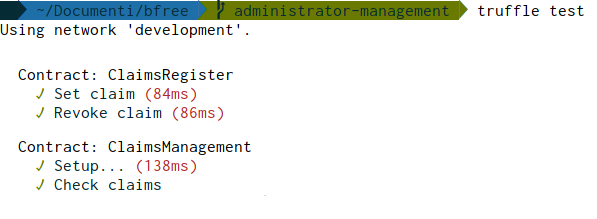
\includegraphics[scale=0.5]{img/test.png}
    \caption{L'esito positivo dei test automatici}
    \label{fig:test}
\end{figure}

\newpage